\documentclass{article}
\usepackage[margin=1in]{geometry}
\usepackage{amsmath,amsthm,amssymb}
\usepackage{bbm,enumerate,mathtools}
\usepackage{tikz,pgfplots}
\usepackage{chessboard}
\usepackage[hidelinks]{hyperref}
\usepackage{multicol} % Problem 35
\usepackage{xstring} % Difficulty command
\usetikzlibrary{shapes.geometric}

\newenvironment{question}{\begin{trivlist}\item[\textbf{Question.}]}{\end{trivlist}}
\newenvironment{note}{\begin{trivlist}\item[\textbf{Note.}]}{\end{trivlist}}
\newenvironment{references}{\begin{trivlist}\item[\textbf{References.}]}{\end{trivlist}}
\newenvironment{related}{\begin{trivlist}\item[\textbf{Related.}]\end{trivlist}\begin{enumerate}}{\end{enumerate}}

\newcommand\score[1]{
\pgfmathsetmacro\pgfxa{#1+1}
\tikzstyle{scorestars}=[
  star,
  star points=5,
  star point ratio=2.25,
  draw,
  inner sep=3pt,
  anchor=outer point 5
]
  \begin{tikzpicture}[baseline]
    \draw[opacity=0] (0,-0.5) rectangle (0,0.2); % Workaround for whitespace at the bottom.
    \foreach \i in {1,...,4} {
      \pgfmathparse{(\i<=#1?"yellow":"gray")}
      \edef\starcolor{\pgfmathresult}
      \draw (\i*4.5ex,0) node[name=star\i,scorestars,fill=\starcolor]  {};
    }
  \end{tikzpicture}
}

\newcommand{\difficulty}[1]{%
  \IfEqCase{#1}{%
      {1}{
        
\begin{tikzpicture}[scale=0.7, baseline=0.9mm]%
          \definecolor{slopegreen}{rgb}{0.0, 0.5, 0.0}%
          \fill[slopegreen] (0.5,0.5) circle (0.5);%
        \end{tikzpicture}%
      }%
      {2}{
        
\begin{tikzpicture}[scale=0.7, baseline=0.9mm]%
          \definecolor{slopeblue}{rgb}{0.0, 0.44, 1.00}
          \fill[slopeblue] (0,0) rectangle (1,1);%
        \end{tikzpicture}%
      }%
      {3}{
\begin{tikzpicture}[scale=0.7, baseline=0.9mm]\fill (0,0.5)--(0.5, 0)--(1,0.5)--(0.5,1)--cycle; \end{tikzpicture}}%
      {4}{
\begin{tikzpicture}[scale=0.7, baseline=0.9mm]\fill (0.25,0)--(0,0.5)--(0.25,1)--(0.5,0.5)--cycle; \fill (0.75,0)--(0.5,0.5)--(0.75,1)--(1,0.5)--cycle;\end{tikzpicture}}%
      % you can add more cases here as desired
  }[\PackageError{difficulty}{Undefined difficulty level: #1}{}]%
}%
\newcommand{\rating}[2]{\difficulty{#1}\\\score{#2}\\}


\begin{document}
\rating{3}{1}
Consider figures created out of ``blocks'' starting from some base state and
with the rule that each new block needs to touch as many old blocks as possible.
\begin{figure}[ht!]
  \centering
  \begin{tikzpicture}[
    level distance=2.5cm,
    sibling distance = 3cm,
    level 1/.style={sibling distance=7cm},
    level 2/.style={sibling distance=2.5cm}
  ]
    \node {
      \begin{tikzpicture}[scale=0.6]
        \draw[fill=blue!50, ultra thick] (0,0) rectangle (1,1);
        \draw[fill=blue!50, ultra thick] (1,0) rectangle (2,1);
      \end{tikzpicture}
    }
    child {
      node {
        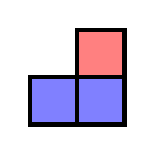
\begin{tikzpicture}[scale=0.6]
          \draw[fill=blue!50, ultra thick] (0,0) rectangle (1,1);
          \draw[fill=blue!50, ultra thick] (1,0) rectangle (2,1);
          \draw[fill=red!50, ultra thick] (1,1) rectangle (2,2);
      \end{tikzpicture}
      }
      child {
        node {
          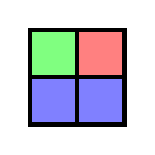
\begin{tikzpicture}[scale=0.6]
            \draw[fill=blue!50, ultra thick] (0,0) rectangle (1,1);
            \draw[fill=blue!50, ultra thick] (1,0) rectangle (2,1);
            \draw[fill=red!50, ultra thick] (1,1) rectangle (2,2);
            \draw[fill=green!50, ultra thick] (0,1) rectangle (1,2);
          \end{tikzpicture}
        }
      }
    }
    child {
      node {
        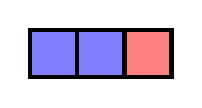
\begin{tikzpicture}[scale=0.6]
          \draw[fill=blue!50, ultra thick] (0,0) rectangle (1,1);
          \draw[fill=blue!50, ultra thick] (1,0) rectangle (2,1);
          \draw[fill=red!50, ultra thick] (2,0) rectangle (3,1);
      \end{tikzpicture}
      }
      child {
        node {
          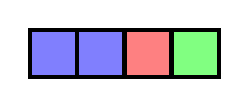
\begin{tikzpicture}[scale=0.6]
            \draw[fill=blue!50, ultra thick] (0,0) rectangle (1,1);
            \draw[fill=blue!50, ultra thick] (1,0) rectangle (2,1);
            \draw[fill=red!50, ultra thick] (2,0) rectangle (3,1);
            \draw[fill=green!50, ultra thick] (3,0) rectangle (4,1);
          \end{tikzpicture}
        }
      }
      child {
        node {
          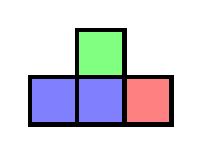
\begin{tikzpicture}[scale=0.6]
            \draw[fill=blue!50, ultra thick] (0,0) rectangle (1,1);
            \draw[fill=blue!50, ultra thick] (1,0) rectangle (2,1);
            \draw[fill=red!50, ultra thick] (2,0) rectangle (3,1);
            \draw[fill=green!50, ultra thick] (1,1) rectangle (2,2);
          \end{tikzpicture}
        }
      }
      child {
        node {
          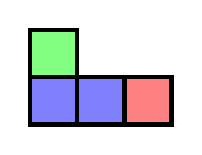
\begin{tikzpicture}[scale=0.6]
            \draw[fill=blue!50, ultra thick] (0,0) rectangle (1,1);
            \draw[fill=blue!50, ultra thick] (1,0) rectangle (2,1);
            \draw[fill=red!50, ultra thick] (2,0) rectangle (3,1);
            \draw[fill=green!50, ultra thick] (0,1) rectangle (1,2);
          \end{tikzpicture}
        }
      }
    };
  \end{tikzpicture}

  \caption{
    On the leftmost path, the final transition is from an ``L'' to a square,
    because the maximum number of faces that can touch is two, so the block must
    be added in the upper left corner.
    Counting the number of vertices gives $a(1) = 1$, $a(2) = 2$, and $a(3) = 4$.
  }
\end{figure}
\begin{question}
  How many distinct figures (up to group action) can be made with $n$ blocks,
  always following a greedy algorithm (with respect to number of faces touching)?
\end{question}

\begin{related}
  \item What if this is done with circles on a hexagonal grid? (Polyiamonds, etc.)
  \item What if this is done in more than $2$ dimensions?
  \item What if the starting shape is different? (e.g. the ``T'' tetromino)
  \item What if the blocks are different? (e.g. dominoes)
  \item What if the constraint is changed? (e.g. each block must touch exactly two sides)
\end{related}

\begin{references}
  \item Problem 65
\end{references}
\end{document}
